% status: TBD
% chapter: TBD

\title{Orange}


\author{Moeen Arshad}
 \affiliation{%
  \institution{Indiana University Bloomington}
  \city{Bloomington} \state{Indiana}  \postcode{47408}
  }
\email{marshad@iu.edu}

\renewcommand{\shortauthors}{G. v. Laszewski}

\begin{abstract}

Orange is a data mining, visualization, and machine learning toolkit
based on Python 3. Built at the University of Ljubljana, Slovenia by
the Faculty of Computer and Information Science utilizing the
Bioinformatics Library, this software was developed to allows domain
experts and data scientists, alike, to take advantage of its capabilities
in order to perform complex data mining and machine learning practices.
Orange is targeted towards practitioners with varying degrees of technical
background, including complete novices, and aims to simplify the
product’s offerings through a visualization interface that describes
the workflow in components, otherwise known as widgets.  Capabilities of
this product include the ability to utilize random forests, Naïve Bayes,
neural networks, and k-nearest neighbors for data mining and machine
learning practices. Orange’s data source is typically in tabular format,
with attributes in columns and instances in rows, and the software’s
capabilities can be enhanced by developers who wish to create their
own widgets. Add-ons are also readily available to extend Orange's
functionality in specific domains such as bioinformatics, or text
mining.
\end{abstract}

\keywords{hid-sp18-504, Orange, Machine Learning, Data Mining,
          Visualization}


\maketitle


\section{Introduction}

Developed in a bioinformatics laboratory by a Computer and Information
Science faculty~\cite{hid-sp18-504-predanalytics}, Orange was built for
use by practitioners of all skill levels, ranging from developers to
novices~\cite{hid-sp18-504-predanalytics}.
With an interactive data visualization interface, Orange allows for
a simple approach to perform complex data mining and machine learning
practice through a component based workflow ui. This simplified approach
to utilizing data mining and machine learning practices can be utilized
not only as a tool to bridge the gap between domain experts and data
scientists, but in addition to be leveraged in academic and
research settings. Orange’s visual programming component is presented in
the form of widgets in order to perform qualitative analysis through a
visualized workflow map. This workflow map can have a number of different
widgets included, each grouped into its own clas depending on a widget's
function; which encourages the use of various different types of
widgets mapped together in any given typical workflow. Orange can not only
be utilized as a Python library, but developers can create their own custom
widgets via Python scripting and add it to
their workflow~\cite{hid-sp18-504-orange}.
In addition to Orange being used for various data mining tasks, visualizations,
and machine learning tasks, additional add-ons are available to extend Orange's
functionalities, such as for domains involving ``biomedicine, bioinformatics,
[and] genomic research''~\cite{hid-sp18-504-wiki-orange}.

\section{Design Overview}

This open source toolkit's latest version (3+) uses various python libraries
for computation, while utilizing the Qt framework for the visualization
end~\cite{hid-sp18-504-wiki-orange}.
Orange was initially built atop C++ classes to cover
modeling and preprocessing.
Users interact with the Python layer which uses
``popular Python libraries numpy for linear algebra,
networkx for working with networks and matplotlib for
basic visualization''~\cite{hid-sp18-504-journalorange}.
Orange can integrate with various Python IDEs such as PyCharm or shells such as
iPython, and offers cross-platform support on Windows, Linux, and
MacOS X~\cite{hid-sp18-504-predanalytics}.
The overall interface the user encounters with Orange can be broken down
into two separate features; widgets, which cover Orange’s data mining and
machine learning functionalities, and a canvas interface for users to design
their workflow which links together widgets~\cite{hid-sp18-504-wiki-orange}.
See\label{f:fig1} for an example of a workflow in Orange.

\begin{figure}[!ht]
  \centering
  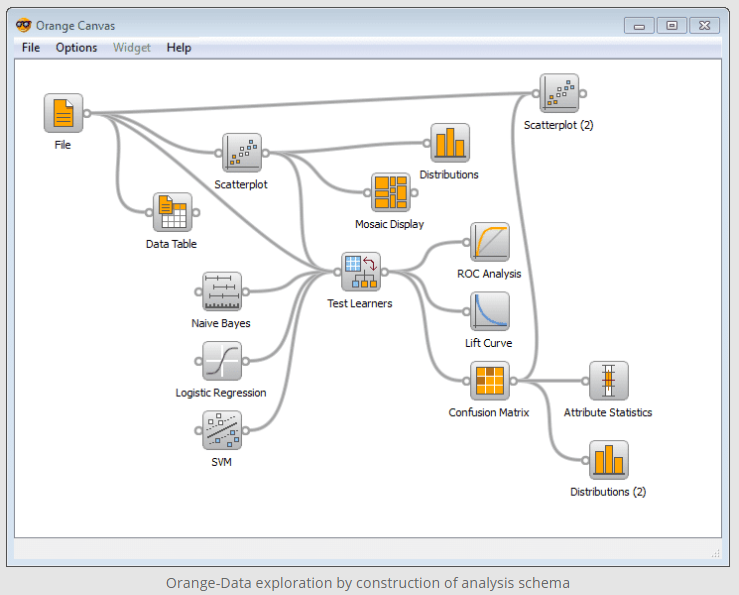
\includegraphics[width=\columnwidth]{images/orangeworkflow-predanalytics.png}
  \caption{Example
  of Orange Workflow~\cite{hid-sp18-504-predanalytics} }
\label{f:fig1}
\end{figure}

\section{Functionality}
Some of Orange's available Python classes and methods
include classes based on data models, preprocessing,
classification, regression, clustering, distance,
evaluation, and projection. The classification and
regression classes offer the largest number of available methods,
such as random forests,Naive Bayes, neural networks,
and k-nearest neighbors~\cite{hid-sp18-504-orange}.
These classes can either be used directly as a Python library, or used
in Orange's widget sets. Users are able to script their own
custom widgets in Python once meta data for the widget
is defined, along with input/output specification, which
are handled by class methods. These custom widgets
can then be aded to the  Orange workflow, which define
some of Orange's key capabilities~\cite{hid-sp18-504-wiki-orange}.

\subsection{Widgets and Add-Ons}
Widgets are the self-contained functional components that
define a workflow's task. Using
communication channels to pass outputs from one widget to another,
data can be processed and transformed  using these self-contained
functionalities to achieve the desired output. Users are capable of
scripting their own functionalities in custom widgets once an input/output
specification has been defined, along with constants for the class
namespace. Users also have the ability to utilize the pre-existing
widgets that are packaged with the software~\cite{hid-sp18-504-orange}.

Add-ons are utilized for targetted research, which extend Orange's
functionality. Add-ons that are offered with
Orange include Bioinformatics,
Network, Spark, and Text, which can be simply added to Orange by
navigating to the Options menu. These add-ons can be used in conjunction
with Orange's existing widget set~\cite{hid-sp18-504-orange}.

The current widget catalog~\cite{hid-sp18-504-orange}, including some
of the available add-ons, can be categorized as the following:

\begin{itemize}

   \item {\bf Data} (define data sources, perform
   transformations, preprocess)
   \item {\bf Visualize} (utilize various visualizations such as heat maps,
   linear projections, and Pythagorean forests)
   \item {\bf Model} (implement algorithms such as Naïve Bayes, neural
   networks, linear regression, kNN)
   \item {\bf Evaluate} (perform predictions and plot analysis)
   \item {\bf Unsupervised} (implement algorithms such as k-Means, distance
   transformation, correspondence analysis)
   \item {\bf Data Fusion} (construct data fusion graphs and relation matrices)
   \item {\bf Educational} (designed for educational purposes such as
   interactive k-Means and polynomial classification)
   \item {\bf Text} (offers various text based sources)
   \item {\bf Network} (offers functionality for network analysis)
   \item {\bf Bioinformatics} (various components related to bioinformatics,
   such as gene info and KEGG Pathways)
   \item {\bf Associate} (offers associate rules and frequent item sets)

\end{itemize}

\subsection{Data Sources}
Using the File Widget, Orange is capable of importing native files,
csv’s, text files, Excel spreadsheets, or Google Sheets.
In short, the data that
is consumed by Orange is typically in tabular format defined as samples
by attributes, or rows by columns. Attributes can be defined as one of
four category types: discrete, time, continuous, or string. Orange will
make assumptions of attribute roles and types when importing data, but
corrections can be made once again by utilizing the File Widget.
For performance and compatibility (such as with scikit-learn),
Orange wraps its datasets in numpy arrays, which allows details of
the values and feature names to be stored~\cite{hid-sp18-504-orange}.

\subsection{Classification}
Supervised data mining, or classification, is a primary focal point of
Orange's machine learning methods, which are dependent on class-labeled
instances. These classifiers are comprised of two different object types,
learner and classifiers~\cite{hid-sp18-504-orange}; where learners consume
class-labeled data in order to return classifiers. Many different learners
can be used on the same dataset, each with varying
parameters to distinguish
one learner from another and provide unique feedback, which are further
utilized in ensembles, which are implemented as wrappers around various
learners~\cite{hid-sp18-504-predanalytics}.

To further enrich the classification methods that are offered, the following
types of classification can be utilized in Orange~\cite{hid-sp18-504-orange}:

\begin{itemize}

   \item {\bf Probabilistic Classification} (classifier that is called using
   additional parameters in order to specify a classification based on output)
   \item {\bf Cross Validation} (this method is used to validate the accuracy
   of a classification by averaging the result across several runs of
   classification from the dataset)
   \item {\bf Classifiers} (scikit-learn is utilized to offer a number of
   different classifiers in Orange which include logistic regression, kNN,
   support vectore machines, classification trees, and random forests)

\end{itemize}

\subsection{Regression}
Regression, similiar to classification, is also dependent on class-labeled
data, and is implemented using learners and regressors. In short, regression
models, or regressors, predict a continous class value based on an input.
Also similiar to classification, there are a number of available regressors
in Orange (such as neural network, regression trees, linear regression, and
polynomials), and cross validation is also a good way of checking a regression
scoring method~\cite{hid-sp18-504-orange}.

\section{Support}
Orange is open source, and is released under
GPL~\cite{hid-sp18-504-journalorange}.
This toolkit is cross-platform, and supports Windows, Mac OS and
Linux~\cite{hid-sp18-504-wiki-orange}.
``As of March 2018 the stable version is 3.11 and runs with Python 3,
while the legacy version 2.7 that runs with
Python 2.7 is still available''~\cite{hid-sp18-504-wiki-orange}.
Orange’s installer comes packaged with
Anaconda~\cite{hid-sp18-504-analyticsvidhya}, and the GUI requires a
PyQt installation~\cite{hid-sp18-504-orange}. Users may also install
Orange directly from the Python Package Index
repository~\cite{hid-sp18-504-journalorange}. Given t
hat Orange is a free
software released under the terms of the GNU General Public License,
Orange does not offer any warranty on the product.


\section{Conclusion}

Using a canvas-based workflow diagram with functional widget components,
Orange offers a solution which simplifies the process of data mining,
machine learning, and visualization, and makes it accessible to users with
novice technical backgrounds. This toolkit allows domain experts the ability
to take advantage of powerful data-science rooted analytic methods; methods
which traditionally were available to practitioners of
data science with a strong
technical background. Friendly towards experts as well, Orange’s
Python-based
functionalities offer users the ability to utilize a large number of existing
Python libraries and integrate with various IDEs and shells. Users also have
the flexibility to develop custom widgets using Python scripts with support
for Python 2.X and Python 3.X. Orange also has a number of add-ons available,
which include bioinformatics-based enhanced functionalities. This open
source software has gathered an audience in research and academic
settings due to its ease of use and simply entry into practicing
data mining and machine learning techniques. In addition, Orange
has accumulated several add-ons, which include bioinformatics
and text mining; and is thus known in the bioinformatics
domain space, as well. 


\begin{acks}

  The authors would like to thank Dr.~Gregor~von~Laszewski for his
  support and suggestions to write this paper.

\end{acks}

\bibliographystyle{ACM-Reference-Format}
\bibliography{report}
